\documentclass[4apaper,11pt,fleqn]{article}

% package imports
% ---------------

\usepackage[british]{babel} % for correct language and hyphenation and stuff
\usepackage{enumitem}       % for configuring list environments
\usepackage{fancyhdr}       % for setting header and footer
\usepackage{geometry}       % for setting margins (\newgeometry)
\usepackage{graphicx}       % for pictures
\usepackage{microtype}      % for microtypography stuff
\usepackage{xcolor}         % for colours
\usepackage{amsmath}        % improve math presentation
\usepackage{amssymb}	      % math's symbols
\usepackage{amsfonts}       % standard math's amsfonts
\usepackage{mathtools}      % for improved notation
\usepackage{amsthm}         % for def, theorems etc.
\usepackage[hidelinks]{hyperref}

% definition and remarks
% ------------

\theoremstyle{remark}
\newtheorem*{rem}{Remark}
\theoremstyle{definition}
\newtheorem*{dfn}{Definition}

% fancyness for the page
% -----------------

\pagestyle{fancy}                 % for select a style
\fancyhf{}                        % for emptying the head and the foot
\rhead{\nouppercase{\leftmark}}   % print on the right head the current section name and number (for article)
\lfoot{\thepage}                  % page number on the lower right part


% main document
% ----------------

% title
\title{Notes about Complex Systems' presentation}
\author{Leonardo Salicari}
%\date{}

\begin{document}

% title and table of content
\maketitle
\tableofcontents


% Ch 1.5.2
% ---------------
\section{Discrete: Isotropic RW with 2 absorbing barriers}
\begin{dfn}[Absorbing barrier]
  An absorbing barrier is a state $i$ such that in the corresponding Markov Chain (MC) has $W_{ii} = 1$.
  Hence, from normalization, $W_{ji} = 0 \quad \forall  j \neq i$.
\end{dfn}
Setup: we have a 1D random walker in a system of $N$ discrete points. Both in $1$ and $N$ we have absorbing barriers. The corresponding transition probability matrix is the follow:
\begin{align*}
  W = \left( \begin{array}{ccccccccc}{1} & {1-r} & {0} & {0} & {0} & {\cdots} & {0} & {0} & {0} \\ {0} & {0} & {1-r} & {0} & {0} & {\cdots} & {0} & {0} & {0} \\ {0} & {r} & {0} & {1-r} & {0} & {\cdots} & {0} & {0} & {0} \\ {0} & {0} & {r} & {0} & {1-r} & {\cdots} & {0} & {0} & {0} \\ {\vdots} & {\vdots} & {\vdots} & {\vdots} & {\vdots} & {\ddots} & {\vdots} & {\vdots} & {\vdots} \\ {0} & {0} & {0} & {0} & {0} & {\cdots} & {0} & {r} & {1} \end{array} \right)
\end{align*}
where $ W_{i+1,i} = r $ and $W_{i-1,i} = 1-r$. Note the absorbing conditions on 1 and $N$.
\begin{rem}
  Also note the convention on indices: the row index, the first one form the left, is relative to the final state while the column index, the second one, is relative to the initial state.
\end{rem}
For any $j \in [1,N] \subset \mathbb{N}$ the walker has probability 1 to be absorbed by one of the barriers at some point in time\footnote{See P. Brémaud, "Markov chains".}. We can conclude that from the structure of $W$ the MC is irreducible but apart of the persistent states 1 and $N$ all others are transient
\begin{dfn}
  A MC is said to be \emph{irreducible} if all states are accessible from any other states. Formally, there exist a $t$ such that $W^t_{j,i} > 0 \quad \forall j, i$.\\
  A state $i$ is said to be \emph{persistent} if $W_{i,i}=1$. On the other hand, is said to be \emph{transient} if $W_{i,i}<1$.
\end{dfn}

Which is the probability that a RW starting in $j$ will reach 1 without being absorbed by $N$?\\
Let $p_j =$ time-dependent prob to be trapped at 1 given that the RW started in $j$ at $t=0$. For $j \in [2,N-1]$ it obeys the equation:
\begin{align}
  \label{eq:pj}
  p_{j} &=W_{j+1, j} \, p_{j+1} + W_{j-1, j}\, p_{j-1} \\ \notag
  &=r\, p_{j+1}  + (1-r)\, p_{j-1}
\end{align}
which has the same formal structure of the update rule for the probability distribution of a RW on a ring but with the boundary conditions $p_1 = 1$ and $p_N = 0$, because of its definition.
Note also that $W$ is actually a transition rate when considering discrete and unitary time steps, as in our case.\\
A simple derivation of \eqref{eq:pj} is given in the book "Probability and Random Processes" by G. R. Grimmett and D. R. Stirzaken\footnote{Chap. 1.7, example 4, "Symmetric random walk" or "Gambler's ruin".}: Let $A$ be the event for which the walker is absorbed in 1 and $B$ the event related to take a step on the right, a.k.a. $j\rightarrowj+1$. Let $\mathbb{P}_k(A)$ the probability of $A$ given that we are in the $k$ state (position), hence we can write, denoting the universe space as $\Sigma$:
\begin{align*}
  \mathbb{P}_{k}(A) &= \mathbb{P}_k (A \cap \Sigma) = \mathbb{P}_k (A \cap (B \cup B^c) ) = \mathbb{P}_k ( (A\cap B ) \cup ( A \cap B^c ) ) \\
                    &= \mathbb{P}_{k}(A | B) \mathbb{P}_k (B)+\mathbb{P}_{k}\left(A | B^{c}\right) \mathbb{P}_k \left(B^{c}\right)
\end{align*}
Now we look into the detail of $\mathbb{P}_{k}(A | B)$, probability to be absorbed in 1 given that the walker jumped into $k+1$ state; basically, after the walker go to the state $k+1$ we have to compute the probability that, from $k+1$ position, the walker is absorbed in 1. But this is exaclty $\mathbb{P}_{k+1} (A)$, thus $\mathbb{P}_{k}(A | B) = \mathbb{P}_{k+1} (A)$. Similarly $\mathbb{P}_{k}(A | B^c) = \mathbb{P}_{k-1} (A)$, given that $B^c$ represent the event in which the walker goes to its left, a.k.a. $k-1$.
Lastly, we can identify $\mathbb{P}_k (B) = W_{k+1,k}$ and this proves \eqref{eq:pj}.


% solution to the equation
\subsection{Solutions for $r=1/2$ and $r\neq 1/2$}
As we have done the RW on a ring case, we assume $p_k = \psi^k$, i.e the parameter $\psi$ to the $k$, hence
\begin{align*}
  \psi^j = r\psi^{j+1} + (1-r) \psi^{j-1} \quad \Rightarrow \quad 0 = r\psi^2 - \psi + (1-r)
\end{align*}
which has the solutions (just substitute):
\begin{itemize}[leftmargin=*]
  \item $\psi_1 = 1 \Rightarrow p_j^{(1)} = 1$
  \item $\psi_2 = (1-r)/r := s \Rightarrow  p_j^{(2)} = s^j$
\end{itemize}
\begin{rem}
  This solutions are such thanks to the ansatz $p_k = \psi^k$
\end{rem}
These are degenerate when $r=1/2$; in this case it appears another solution which is $p_j^{(2)} = j$ (here we are calling 2 the second non degenerate solution). This is a solution because the equation \eqref{eq:pj} becomes $p_j = (p_{j+1}+p_{j-1})/2$.\\
For $r\neq1/2$, a.k.a. \emph{asymmetric case}, the general solution of the equation is given by the linear combination of independent solutions, hence:
\begin{align*}
  p_j^{as} = As^j + B
\end{align*}
where $A$ and $B$ are constants which are fixed by the boundary conditions:
\begin{align*}
   &p_1^{as} = As + B = 1\\
   &p_N^{as} = As^N + B = 0\\
   &\Rightarrow A= \frac{1}{s(1-s^{N-1})} \qquad B = - \frac{s^{N-1}}{(1-s^{N-1})}
\end{align*}
Thus the solution for the asymmetric case is
\begin{align}
  \boxed{p_j^{as} = \frac{s^{j-1}-s^{N-1}}{1-s^{N-1}}}
\end{align}
\begin{rem}
  This is the one, together with the symmetric solution, that will be tested numerically
\end{rem}

For $r=1/2$, a.k.a. \emph{symmetric case}, the general solution is, as before, a linear combination,
\begin{align*}
    p_j^{s} = A \, j + B
\end{align*}
and the boundary conditions gives:
\begin{align*}
  A = -\frac{1}{N-1} \qquad B = \frac{N}{N-1}
\end{align*}
resulting the the solution for the symmetric case:
\begin{align}
  \label{eq:solS}
  \boxed{p_j^{s} = \frac{N-j}{N-1}}
\end{align}

% thermo limit
\subsection{Thermo limit}
For $r>1/2$ (or $s<1$) and in the limit $N \rightarrow \infty$, we have:
\begin{align}
  \label{eq:asym_limit}
  A = 1/s \qquad B = 0 \qquad \Rightarrow \qquad \boxed{p_j^{\text{thermo}} = s^{j-1}}
\end{align}
hence the probability of being absorbed in 1 starting at $j$ decreases exponentially with $j$ because the system has a bias ($r>1/2$) toward the other absorbing barrier with is at infinity. On the other hand, if $r<1/2$ we have $p_j=1 \quad \forall j$ because the system is driven toward the absorbing 1 state. Stated in other words, eventually the RW will remain trapped in 1.\\
The same conclusion can be drawn for $r=1/2$ because the unbiased RW is such that any state is visited from any other in a finite amount of time, i.e. from every $j$ eventually one arrives at 1. This can be seen by the symmetric solution or by showing that the unbiased RW is an irreducible MC.
Hence we can conclude:
\begin{align*}
  p_j = 1 \qquad r \leq \frac{1}{2} \quad \text{and} \quad N \rightarrow \infty
\end{align*}


% Ch 1.6.3
% ---------------
\section{Continuum: Stationary Isotropic RW with 2 absorbing barriers}
In the context of continuous time ad space stochastic processes we can introduce as a continuous approximation, in space and time, for the master equation the Fokker-Planck equation.
Without entering into details, the general form of the FP equation for the probability density $P(X,t)$ is the following:
\begin{align*}
  \frac{\partial P(X, t)}{\partial t}=-\frac{\partial}{\partial X}(a(X, t) P(X, t))+\frac{1}{2} \frac{\partial^{2}}{\partial X^{2}}\left(b^{2}(X, t) P(X, t)\right)
\end{align*}
where $a(X,t)$ is the generalized drift component while $b(X,t)^2/2$ is the generalized diffusion coefficient.\\
The FP can be express as a continuity eq:
\begin{align}
  \label{eq:continuity}
  \frac{\partial P(X, t)}{\partial t}+\frac{\partial J(X, t)}{\partial X}=0
\end{align}
where
\begin{align*}
  J(X, t)=a(X, t) P(X, t)-\frac{1}{2} \frac{\partial}{\partial X}\left(b^{2}(X, t) P(X, t)\right)
\end{align*}
which can be interpreted as a probability current.
Let $X \in \mathbb{R}$, we consider an interval $I=[X_1,X_2]$ and define the probability that the stochastic process described by \eqref{eq:continuity} is in $I$, $\mathcal{P}(t)$,
\begin{align*}
  \mathcal{P}(t) = \int_I P(X,t) \, dX
\end{align*}
Integrating \eqref{eq:continuity} in $X$, we obtain
\begin{align*}
  \frac{\partial \mathcal{P}(t)}{\partial t}=J\left(X_{1}, t\right)-J\left(X_{2}, t\right)
\end{align*}

This form is quite useful because, usually, in numerical simulation one woks with stochastic processes confined in finite intervals. To this situation, we can apply different boundary conditions:
\begin{itemize}[leftmargin=*]
  \item Reflective barriers\\
  E.g. $J(X_1,t)=J(X_2,t)=0 \quad \forall t$, i.e. zero probability flow outside as well as inside the interval, which correspond to a conservation of the total probability in that interval.
  \item Absorbing barriers\\
  Hence $P(X_1,t) = P(X_2,t) = 0 \quad \forall t$.
  \item Periodic Boundaries\\
  Hence $P(X_1,t) = P(X_2,t)$ and $J(X_1,t)=J(X_2,t)$.
\end{itemize}


% stationary solution
\subsection{Stationary solution in the diffusive case}
The stationary distrbution $P^{*}(X)$ is defined as:
\begin{align}
  \label{eq:dx_flux}
  &\frac{\partial P(X, t)}{\partial t} = 0 \quad \Rightarrow \quad \frac{\partial J(X, t)}{\partial X}=0 \\ \notag
  &\Rightarrow \quad \frac{d}{d X}\left(a(X) P^{*}(X)\right)-\frac{1}{2} \frac{d^{2}}{d X^{2}}\left(b^{2}(X) P^{*}(X)\right)=0
\end{align}
Note that here we have only total derivatives. Moreover, it was assumed that $a(X)$ and $b(X)$ don't depend on time anymore.
Now we consider the case in which $a = 0$ and $b^2 =2D$ a.k.a. the \emph{diffusive case}; the general solution is given integrating two times w.r.t. $X$ obtaining:
\begin{align}
  \label{eq:statSol}
  P^*(X) = C_1 X + C_2
\end{align}
where $C_1, C_2$ are constant to be determine by boundary and normalization conditions.

Let's consider \emph{reflective boundaries}.\\
The continuity equation reads:
\begin{align*}
  J^* (X_i) = -D \frac{d }{d X} P^*(X_i) = 0
\end{align*}
for $i = 1,2$. From \eqref{eq:statSol} we have $C_1 = 0$ and considering the normalization in $I$
\begin{align*}
  \int_{X_1}^{X_2} P^* (X) \, dX = C_2 (X_2 - X_1) = 1 \quad \Rightarrow \quad C_2 = (X_2 - X_1)^{-1}
\end{align*}
Hence, in this case, the stationary probability is a constant. This is equivalent to the periodic boundary conditions and so it's related to the solution for the discrete RW in a ring; to obtain the result we must impose $J(X_1)=-J(X_2)$, i.e. all outgoing flux is equal but opposite in sign to the ingoing flux from the other extreme, and the normalization.

Let's consider \emph{absorbing barriers}\\
If both extrema are absorbing, then $P^*$ is identically zero. This because we have the system:
\begin{align*}
  &C_1 X_1 + C_2 = 0 \\
  &C_1 X_2 + C_2 = 0
\end{align*}
which has solution $C_1 = C_2 = 0$ and it's the only one because the coefficient matrix is non-singular. This reflect the fact that, at infinite time, the random walk eventually encounters an absorbing barrier. \\
A more interesting situation is when we consider a \emph{set} of random walkers. Basically we inject at each time step a random walker in $X_0 \in I$, generating a flux of random walkers.
In this case, the general solution for the stationary distribution is
\begin{align*}
  P^{*}(X)=\left\{\begin{array}{ll}{C_{1}\left(X-X_{1}\right),} & {\text { for } X<X_{0}} \\
  {C_{2}\left(X_{2}-X\right),} & {\text { for } X>X_{0}}\end{array}\right. % the . is an invisible character to counter balance the \left and \right's
\end{align*}
because it satisfy the boundary conditions $P^*(X_1)=P^*(X_2)=0$. The probability distribution has to be continuous in $X_0$, hence the following must be satisfied:
\begin{align*}
  C_{1}\left(X_{0}-X_{1}\right)=C_{2}\left(X_{2}-X_{0}\right)
\end{align*}
The extra flux has to be taken into account in the continuity equation:
\begin{align*}
  \frac{\partial P(X, t)}{\partial t}+\frac{\partial J(X, t)}{\partial X}= F \, \delta (X - X_0)
\end{align*}
In the stationary case, $\partial_t P(X,t) = 0$, we have that the flux must satisfy:
\begin{align*}
  F &= \int_{X_0 - \varepsilon}^{X_0 + \varepsilon} \partial_X J \, dX  \\
    &= -D \left[ \frac{d P^*}{dX}\Bigr|_{X_0 + \varepsilon} - \frac{d P^*}{dX}\Bigr|_{X_0 - \varepsilon} \right] \\
    &= D [C_1 + C_2]
\end{align*}
The latter along with the continuity constrain for the $P^*$ gives a non-homogeneous system for $C_1$ and $C_2$ which has solutions:
\begin{align*}
  C_1 = \frac{F}{D} \frac{X_2 - X_0}{X_2 - X_1} \qquad C_2 = \frac{F}{D} \frac{X_0 - X_1}{X_2 - X_1}
\end{align*}
Finally the stationary solutions for the density probability and for the current are, defining $L_+ = X_2-X_0$ and $L_- = X_0-X_1$ and $L = X_2-X_1$:
\begin{align*}
  P^{*}(X)=\left\{\begin{array}{l}{\frac{F}{D} \frac{L_{+}}{L}\left(X-X_{1}\right)} \vspace{5pt} \\
  {\frac{F}{D} \frac{L_{-}}{L}\left(X_{2}-X\right)}\end{array}\right.
\end{align*}
\begin{align*}
  J^{*}(X)=\left\{\begin{array}{ll}{-F \frac{L_{+}}{L} := -J_{-},} & {\text {for } X<X_{0}} \vspace{5pt}\\
  {F \frac{L_{-}}{L} := J_{+},} & {\text {for } X>X_{0}}\end{array}\right.
\end{align*}
Basically, $J_-$ and $J_+$ represent the fluxes of random walkers being absorbed at $X_1$ and $X_2$ respectively which satisfy the conservation of "particles" $J_+ + J_- = F$.

\subsection{Probability to leave from $X_1$}
In this framework we can introduce the probability that a particle, starting from $X_0$, is absorbed at $X_1$:
\begin{align}
  \label{eq:prob_absorbing_FP}
  \Pi\left(X_{1} | X_{0}\right)=\frac{J_{-}}{F}=\frac{L_{+}}{L}=\frac{X_{2}-X_{0}}{X_{2}-X_{1}}
\end{align}
which is basically the exit flux from $X_1$ divided by the injected flux $F$.
\begin{rem}
  We obtained a restatement of \eqref{eq:solS} considering the continuous approach given by the FP equation.
\end{rem}
Moreover one can obtain the average exit time from $X_1$ by considering the total number of random walkers divided by the total current flow out, a.k.a $F$.


% D.5
% -------------------
\section{Continuum: Isotropic RW with 1 absorbing barrier}
The FP associated to a 1D RW with  probability density distribution $p(x,t)$ is
\begin{align*}
  \frac{\partial p}{\partial t}=D \frac{\partial^{2} p}{\partial x^{2}}
\end{align*}
With the initial condition $p(x,0)=\delta(x-x_0)$ where $x_0 = x(0)$, the solution to the latter is a gaussian:
\begin{align*}
  p_{x_{0}}(x, t)=\frac{1}{\sqrt{4 \pi D t}} \exp \left(-\frac{\left(x-x_{0}\right)^{2}}{4 D t}\right)
\end{align*}
Note: this can be obtained by Fourier transforming the diffusion equation into the $\vec{k}$ space, impose the initial condition and go back to the real space.

Let's introduce a trap in $x_t = 0$.
\begin{dfn}
  A trap, or absorbing barrier, in $x_t$, is defined as the point in which $p(x_t,t)=0 \quad \forall t$.
\end{dfn}
This condition is satisfied by taking a linear combination of the previous solution such that:
\begin{align}
  \label{eq:sol_trap}
  p(x, t)=\frac{1}{\sqrt{4 \pi D t}}\left[\exp \left(-\frac{\left(x-x_{0}\right)^{2}}{4 D t}\right)-\exp \left(-\frac{\left(x+x_{0}\right)^{2}}{4 D t}\right)\right]
\end{align}
which satisfy the definition. A plot for a fixed time is the one in figure \ref{fig:rwiso}.
\begin{figure}
  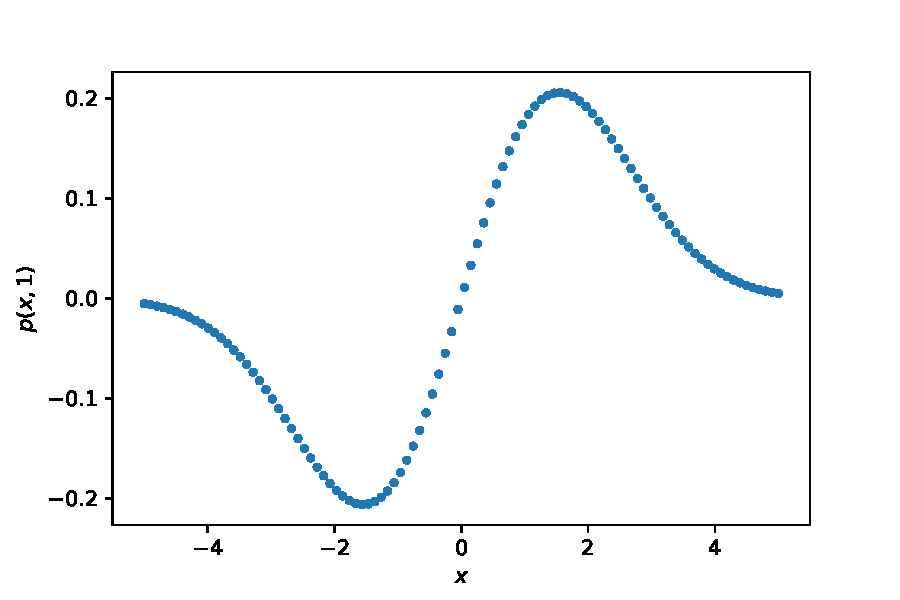
\includegraphics[width=\textwidth]{plot_iso_RW.pdf}
  \caption{Probability distribution for the Isotropic RW with a trap in $x_t=0$.}
  \label{fig:rwiso}
\end{figure}

\subsection{First passage probability}
The first passage probability $f(t)$ is the probability that the particle is trapped in $x_t=0$ in the time interval $[t,t+dt]$ and it's equal to the module of the current $|J|$ evaluated at $x_t$.
Basically, this has a similar interpretation to the stationary probability for a set of random walkers to be absorbed in an absorbing barrier, i.e. equation \eqref{eq:prob_absorbing_FP}.
Hence using \eqref{eq:sol_trap}:
\begin{align*}
  f (t) = \left|  J(x,t) \Bigr|_{x=0} \right| = \left|  -D \frac{\partial p(x,t)}{\partial x}\Bigr|_{x=0} \right| = \frac{x_{0}}{\sqrt{4 \pi D t^{3}}} \exp \left(-\frac{x_{0}^{2}}{4 D t}\right)
\end{align*}
A quick check, by integrating over time from 0 to $\infty$ (using the change of variable $\tau^2 = x_0^2/4Dt$), conferm that the probability is normalized. \\
Note: the average trapping time, time in which the particle is \emph{not} absorbed, $\langle t_t \rangle$ is divergent because for large $t \Rightarrow t\,f(t) \sim 1/\sqrt{t}$ and the definition is:
\begin{align*}
  \langle t_t \rangle = \int_0^\infty t \, f(t) \, dt \sim \infty
\end{align*}
Nevertheless,  the \emph{median} trapping time $t_{med}$, defined as:
\begin{align*}
  \int_{t_{med}}^\infty f(t)\, dt = \int_0^{t_{med}} f(t) \, dt
\end{align*}

\subsection{Mean position}
\label{subsec:mean_pos}
The mean position $\langle x \rangle$ for this process can be computed as follows:
\begin{align*}
  \langle x(t)\rangle &= \int_{0}^{\infty} d x \frac{x}{\sqrt{4 \pi D t}}\left[\exp \left(-\frac{\left(x-x_{0}\right)^{2}}{4 D t}\right)-\exp \left(-\frac{\left(x+x_{0}\right)^{2}}{4 D t}\right)\right] \\
                      &= \int_{0}^{\infty} d x \frac{x}{\sqrt{4 \pi D t}} \exp \left(-\frac{\left(x-x_{0}\right)^{2}}{4 D t}\right)+\int_{-\infty}^{0} d x \frac{x}{\sqrt{4 \pi D t}} \exp \left(-\frac{\left(x-x_{0}\right)^{2}}{4 D t}\right) \\
                      &= \int_{-\infty}^{\infty} d x \frac{x}{\sqrt{4 \pi D t}} \exp \left(-\frac{\left(x-x_{0}\right)^{2}}{4 D t}\right) \\
                      &= x_0
\end{align*}
where we performed the change of variable $x \rightarrow -x$ in the second integral of the first equality.
\begin{rem}
  Notice that the mean position over time doesn't change with the presence of a trap. Hence it remains constant $\boxed{\langle x(t)\rangle = x_0}$.
\end{rem}


% D.5 anisotropic
% -----------------
\section{Continuum: Anisotropic RW with 1 absorbing barrier}
We consider a RW with a negative drift term, i.e. $-v $ where $v>0$ hence the RW tends to move toward left. This is described by the FP:
\begin{align*}
  \frac{\partial p}{\partial t}=v \frac{\partial p}{\partial x}+D \frac{\partial^{2} p}{\partial x^{2}}
\end{align*}
Assuming the initial condition $p(x,0)=\delta (x-x_0)$  and no traps, the solution is given by:
\begin{align}
  \label{eq:sol_drift}
  p_{x_{0}}(x, t)=\frac{1}{\sqrt{4 \pi D t}} \exp \left(-\frac{\left(x-x_{0}+v t\right)^{2}}{4 D t}\right)
\end{align}
This can be obtained as in the case of the diffusion equation.\\
Let's introduce a trap in $x_t=0$. In this case the solution  can be abtained as in the previous chapter, by linearly combining the solution \eqref{eq:sol_drift} to satisfy the condition $p(0,t)=0$ for any time.
Hence:
\begin{align*}
  p(x, t)=\frac{1}{\sqrt{4 \pi D t}}\left[\exp \left(-\frac{\left(x-x_{0}+v t\right)^{2}}{4 D t}\right)-\exp \left(\frac{v x_{0}}{D}\right) \exp \left(-\frac{\left(x+x_{0}+v t\right)^{2}}{4 D t}\right)\right]
\end{align*}
Note the different signs in $x_0$.


\subsection{First passage time}
As before, the probability to be absorbed in the time interval $[t,t+dt]$ $f(t)$ is defined as the module of the current evaluated in $x_t=0$. Since we have a drift term, the current is, see equation \eqref{eq:dx_flux}:
\begin{align*}
  J(x,t) = -v\, p(x,t) -D \frac{\partial p}{\partial x}
\end{align*}
Thus:
\begin{align*}
  f (t) &= \left|  J(x,t) \Bigr|_{x=0} \right| = D \left| \frac{\partial p}{\partial x} \Bigr|_{x=0} \right| \\
        &= \frac{D}{\sqrt{4 \pi D t}}\left[\exp \left(-\frac{\left(x_{0}-v t\right)^{2}}{4 D t}\right) \frac{\left(x_{0}-v t\right)}{2 D t}+ \exp \left(\frac{v x_{0}}{D}\right) \exp \left(-\frac{\left(x_{0}+v t\right)^{2}}{4 D t}\right) \frac{\left(x_{0}+v t\right)}{2 D t}\right] \\
        &= \frac{x_{0}}{\sqrt{4 \pi D t^{3}}} \exp \left(-\frac{\left(x_{0}-v t\right)^{2}}{4 D t}\right)
\end{align*}

Now we want to compute the probability that the particle is absorbed within $t$, which is basically the integral from 0 to $t$ of $f(t)$. Hence:
\begin{align*}
  \int_0^t f(t) \, dt &= \frac{x_{0}}{\sqrt{4 \pi D}} \exp \left(\frac{x_{0} v}{2 D}\right) \int_{0}^{t} \frac{d t^{\prime}}{\left(t^{\prime}\right)^{3 / 2}} \exp \left(-\left(\frac{x_{0}^{2}}{4 D} \frac{1}{t^{\prime}}+\frac{v^{2}}{4 D} t^{\prime}\right)\right) \\
                      &= \frac{2}{\sqrt{\pi}} e^{c} \int_{\bar{u}}^{\infty} d u \exp \left(-\left(u^{2}+\frac{c^{2}}{4 u^{2}}\right)\right)
\end{align*}
where $\bar{u} = x_0/\sqrt{4Dt}$ and $c= v x_0/2D$ and the last passage is done using the substitution $u^2=x_0^2/4Dt^'$.
For the latter integral, we introduce the \emph{error function} erf$(t)$ which is defined for $c>0$:\footnote{See "Handbook of mathematical functions" edited by M. Abramowtz and I. A. Stegun, eq 7.4.33; in this case we the fact that erf is a odd function for the second term in the r.h.s.}
\begin{align*}
  \int d u \exp \left(-\left(u^{2}+\frac{c^{2}}{4 u^{2}}\right)\right)=\frac{\sqrt{\pi}}{4}\left[e^{c} \operatorname{erf}\left(\frac{c}{2 u}+u\right)-e^{-c} \operatorname{erf}\left(\frac{c}{2 u}-u\right)\right]
\end{align*}
Hence we get:
\begin{align}
  \label{eq:erf}
  \int_0^t f(t) \, dt =  \frac{e^{c}}{2}\left\{e^{c}\left[1-\operatorname{erf}\left(\frac{c}{2 \bar{u}}+\bar{u}\right)\right]+e^{-c}\left[1+\operatorname{erf}\left(\frac{c}{2 \bar{u}}-\bar{u}\right)\right]\right\}
\end{align}
where $\operatorname{erf}(\infty)=1$ is used.
For $t \rightarrow \infty$ we have $\bar{u} \rightarrow 0$, hence the previous becomes $\int_0^\infty f(t) dt = 1$, as it should be. Note, this is true for every $v$, i.e. for every $c>0$.

We now want to consider the equation \eqref{eq:erf} in the $t \gg 1$ limit.\\
In this case $1/\bar{u}\rightarrow \infty$ and the argument of the $\operatorname{erf}(x)$ function diverges. We use the asymptotic behavior:
\begin{align*}
  \operatorname{erf}(x) \simeq 1-\frac{e^{-x^{2}}}{\sqrt{\pi} x}, \quad \text { for } \quad x \rightarrow+\infty
\end{align*}
Getting in the limit of $\bar{u} \rightarrow 0$,
\begin{align*}
 \int_{0}^{t} d t^{\prime} f(t') & \simeq 1+\frac{e^{c}}{2 \sqrt{\pi}} \exp \left(-\frac{c^{2}}{4 \bar{u}^{2}}\right)\left[\frac{1}{\frac{c}{2 \bar{u}}+\bar{u}}-\frac{1}{\frac{c}{2 \bar{u}}-\bar{u}}\right] \\ & \simeq 1-\frac{4}{\sqrt{\pi}} \frac{e^{c}}{c^{2}} \bar{u}^{3} \exp \left(-\frac{c^{2}}{4 \bar{u}^{2}}\right)
\end{align*}
The survival probability $S(t)$ can be obtained as follow, making explicit the expression for $c$ and $\bar{u}$,
\begin{align*}
  S(t) := 1- \int_0^t f(t') \, dt' \simeq \frac{2}{\sqrt{\pi}} \frac{x_{0} \sqrt{D}}{v^{2}} \frac{e^{\frac{v x_{0}}{2 D}}}{t^{3 / 2}} \exp \left(-\frac{v^{2}}{4 D} t\right)
\end{align*}

\subsection{Average time before being trapped}
\label{sebsec:t_trapp}
Let's compute the average time before being trapped:
\begin{align*}
  \left\langle t_{\mathrm{rr}}\right\rangle &=\int_{0}^{\infty} dt\; t f(t)=\frac{x_{0}}{\sqrt{4 \pi D}} \int_{0}^{\infty} \frac{d t}{\sqrt{t}} \exp \left(-\frac{\left(x_{0}-v t\right)^{2}}{4 D t}\right) \\ &=\frac{x_{0}}{\sqrt{4 \pi D}} \exp \left(\frac{x_{0} v}{2 D}\right) \int_{0}^{\infty} \frac{d t}{\sqrt{t}} \exp \left(-\left(\frac{x_{0}^{2}}{4 D} \frac{1}{t}+\frac{v^{2}}{4 D} t\right)\right) \\ &=\sqrt{\frac{x_{0}^{3}}{\pi D v}} \exp \left(\frac{x_{0} v}{2 D}\right) K_{1 / 2}\left(\frac{x_{0} v}{2 D}\right)
\end{align*}
where $K_{1 / 2}(x)$ is the modified Bessel function of the second kind.
For small asymmetry in the RW, i.e. small $v$, we have that $K_{1/2}(x) \simeq \sqrt{\pi/(2x)}$. Hence in this case we have:
\begin{align}
  \label{eq:trr}
  \boxed{\left\langle t_{\mathrm{rr}}\right\rangle \simeq \frac{x_0}{v} \exp \left( \frac{x_0v}{2D} \right)} \qquad \text{for} \; v \rightarrow 0
\end{align}


% Compact direct percolation
% ------------------
\section{Compact Directed Percolation (CDP)}

% introduction
\subsection{Introduction}
\emph{This section is not self-consistent, please refer to the course's notes or the reference book for more details. This is meant to summing up the computation of critical exponents in the universality class of CDP, which is different from the one of DP, using the tools developed in the previous sections.}

The DCP evolution can be mapped to the evolution of the domain walls thanks to the fact that $P(0|1,1)=0$, because $q=0$ and where $P(i|i-1,i+1)$ is the conditional probability of having a certain $s_i(t)$ given the states of $s_{i-1}(t-1)$ and $s_{i+1}(t-1)$\;\footnote{For more details on the notation see the course's notes or the Livi and Politi's book.}. Let $L(t)$ be the number of consecutive active sites at time $t$\;\footnote{This is also called $N(t) := \sum_{i=0}^{\infty} \langle s_i(t) \rangle$.} and let the transition probabilities related to the evolution of the CDP be the following:
\begin{align*}
  &P(1|1,1) = P(0|0,0) = 1, \quad P(0|1,1) = P(1|0,0) = 0, \\
  &P(1|1,0) = P(1|0,1) = p
\end{align*}
Graphically, and try to draw some example, it's easy to see that the update rule for $L(t)$ is:
\begin{align}
  L(t+1)=\left\{\begin{array}{cl}{L(t)+1,} & {\text { with probability } p^{2}} \\ {L(t)-1,} & {\text { with probability }(1-p)^{2}} \\ {L(t),} & {\text { with probability } 2 p(1-p)}\end{array}\right.
\end{align}
$L(t)$, which represent the behavior of domain walls, performes a random walk. In particular we are interested only in the case in which $L(t)$ changes its value. Hence we can defined a random walk for the number of consecutive active sites as a RW within
\begin{align*}
  &\text{Probability to increase by 1 (move to the right)} = r = \frac{p^2}{p^2+(1-p^2)} \\
  &\text{Probability to decrease by 1 (move to the left)}  = 1-r = \frac{(1-p)^2}{p^2+(1-p^2)}
\end{align*}
where the denominator is used for normalization. Note that since $P(0|0,0) = 1$, the state were all the sites are inactive is an absorbing state, because the system remain trapped in that state; the same can be drawn for the state in which all sites are active.\\
In the RW performed by $L(t)$ this translates into an \emph{absorbing state} for $L(t)=0$. Hence we want to apply all the theory previously developed.
\begin{rem}
  For each exponent, related to some observable of the process, we have particular initial conditions (IC), which gives a corresponding meaning to the quantities under investigation.
\end{rem}

% beta' - probability of having at least one active site
\subsection{$\beta^\prime$}
In this context we use as IC only a single sites active at time $t$; hence $L(t)$ represent the width of the cluster at time $t$.\\
We define the order parameter $P(t)$:
\begin{align*}
  P(t) = \langle 1 - \prod_{i=0}^{\infty}(1-s_i(t)) \rangle
\end{align*}
which represent the probability average over different realizations, which have the same IC, to have at least one active site. Rephrasing it the probability to have a cluster at time $t$. In the active phase, i.e. $p \geq p_c = 1/2 $\, \footnote{$P_c=1/2$ because if we apply the transformation $ p \rightarrow 1-p $ and viceversa we obtain another process But exchanging active and inactive site we have that the system is the same of the beginning, i.e. we have a symmetry. Hence the critical point must be the same, thus $p_c=1-p_c \Rightarrow p_C=1/2$. }, and near the critical point in the $t \rightarrow \infty$ limit we have the following behavior:
\begin{align*}
  P(\infty) \sim (p-p_c)^{\beta^\prime}
\end{align*}

Now that we have the behavior in the thermo limit we ask: \emph{which is the probability to grow an infinite cluster in time?}
This in the context of the RW performed by $L(t)$ translates into: what is the probability to not be absorbed by the state $L(t)=0$, a.k.a. all inactive sites?\\
The anwser is given by the discrete biased RW studied in the first section in the thermo limit, basically using the relation \eqref{eq:asym_limit}. Hence the result is:
\begin{align*}
  P(\infty) = 1 - p_2 = 1 - s^1 = 1 - \left(  \frac{1-r}{r}  \right) = \frac{2}{p^2} \left( p - \frac{1}{2} \right) = \frac{2}{p^2} \left( p - p_c \right)
\end{align*}
Note, the absorbing state in \eqref{eq:asym_limit} was in 1, hence the use of $p_2$. Comparing with the definition of the critical behavior, we have that, close to criticality, $\beta^\prime = 1$.

% beta - fraction of active sites
\subsection{$\beta$}
The fraction of active sites is an order parameter defined as
\begin{align*}
  \rho (t) = \frac{N(t)}{L} = \frac{\sum_{i=0}^{\infty} \langle s_i(t) \rangle }{L}
\end{align*}
Using as IC an homogeneous state with a finite $\rho(0)$,  a.k.a. choosing a set of random active sites at $t=0$\;\footnote{This IC are the one used when dealing with this order parameter.}, we have near criticality and for $t\rightarrow \infty$ the following behavior for the fraction of active sites:
\begin{align*}
  \rho(\infty) \sim (p-p_c)^\beta
\end{align*}
Always from $p \geq p_c$. This latter condition is important because in the large time limit this means that tha activity dominates the system leading to all active sites, hence $\rho(\infty) = 1$.
This let us to conclude that $ \beta = 0$.

\begin{rem}
  The fact thaa $\beta$ and $\beta^\prime$ are different is an hallmark for the different universality class respect to the DP class.
\end{rem}


% theta - L(t) as a function of t
\subsection{$\theta$}
For simplicity we use as IC the one active state. The $\theta$ exponent is defined as the time dependence for large time of $L(t)$ \emph{at} criticality, i.e.
\begin{align*}
  L(t)\; \overset{t \gg 1}{\sim} \;t^\theta
\end{align*}
This can be solve looking into the continuum case, as treated in section 3 because The random walk is isotropic, since at criticality $p=p_c=1/2$.\\
The IC $L(0) = 1$ translate into $x_0=1$ while the absorbing state $L(t)=0$ is represented by $x_t=0$. The average of $L(t)$ correspond to the average position of the walker which, as demonstrated in \ref{subsec:mean_pos}, despite the absorbing trap is constant with time. Hence $\theta = 0$.


% ni 's -  correlations
\subsection{$\nu_\perp$ and $\nu_\parallel$}
Near criticality, the space ($\perp$) and time ($\parallel$) correlation lengths diverge as power laws, respectively:
\begin{align*}
  &\xi_{\perp} \sim (p_c-p)^{\nu_\perp} \\
  &\xi_{\parallel} \sim (p_c-p)^{\nu_\parallel}
\end{align*}
In the context of single active site IC and $p \seq p_c$, $\xi_{\perp}$ represent the maximum distance attained before the process dies out and $\xi_{\parallel}$ represent the average lifetime of the walker.

We start by looking at $\xi_{\parallel}$: this can be interpreted as the average time before the walker is trapped. This was computed in \ref{sebsec:t_trapp} in the continuum and in the limit of small drift, a.k.a. small asymmetry toward left.\footnote{Note that the walk is asymmetric in this case because we are looking near the criticality.}
In this approximation we obtained relation \eqref{eq:trr} which reads:
\begin{align*}
  \left\langle t_{\mathrm{rr}}\right\rangle = \xi_{\parallel} \sim v^{-1}
\end{align*}
The drift term is proportional to the asymmetry $\delta$\;\footnote{This can be seen from the derivation of the FP eq. starting from the Master eq. $p_j(t+1)=\sum_{i} W_{ji}p_i(t)$ and going into the continuum with the condition $\lim_{N\rightarrow \infty} (\Delta x/\Delta t) (1 - 2r) = -v$, where $2r-1 = \delta$.} defined as the difference between the prob to hop to the right and the prob to hop to the left:
\begin{align*}
  \delta=\frac{p^{2}-(1-p)^{2}}{p^{2}+(1-p)^{2}}=-\frac{1-2 p}{1+2 p(1-p)} \;\overset{p \rightarrow p_c}{\simeq}\; -\left(p_{c}-p\right)
\end{align*}
Thus
\begin{align*}
  \xi_{\parallel} \sim v^{-1} \sim |\delta|^{-1} \simeq (p_c-p)^{-1}
\end{align*}
hence $\nu_\parallel =1$.

On the other hand, the walker perform a RW, hence the relation between the averaged traveled distance $\xi_{\perp}$ and the time $\xi_{\parallel}$ is
\begin{align*}
  \xi_{\perp} \sim \xi_{\parallel}^{1/2} \sim (p-p_c)^{-1/2}
\end{align*}
impling $\nu_{\perp}=1/2$.

\begin{rem}
  Most of the exponent obtained are equal to the one of the mean field approach of the DP process, with the notable exception $\beta^\prime \neq \beta$.
\end{rem}


\end{document}
